%%%%%%%%%%%%%%%%%%%%%%%%%%%%%%%%%%%%%%%%%
% baposter Landscape Poster
% LaTeX Template
% Version 1.0 (11/06/13)
%
% baposter Class Created by:
% Brian Amberg (baposter@brian-amberg.de)
%
% This template has been downloaded from:
% http://www.LaTeXTemplates.com
%
% License:
% CC BY-NC-SA 3.0 (http://creativecommons.org/licenses/by-nc-sa/3.0/)
%
%%%%%%%%%%%%%%%%%%%%%%%%%%%%%%%%%%%%%%%%%

%----------------------------------------------------------------------------------------
%	PACKAGES AND OTHER DOCUMENT CONFIGURATIONS
%----------------------------------------------------------------------------------------

\documentclass[landscape,a0paper,fontscale=0.285]{baposter} % Adjust the font scale/size here

\usepackage{graphicx} % Required for including images
\graphicspath{{figures/}} % Directory in which figures are stored

\usepackage{amsmath} % For typesetting math
\usepackage{amssymb} % Adds new symbols to be used in math mode
\usepackage{units}

\usepackage{booktabs} % Top and bottom rules for tables
\usepackage{enumitem} % Used to reduce itemize/enumerate spacing
\usepackage{palatino} % Use the Palatino font
\usepackage[font=small,labelfont=bf]{caption} % Required for specifying captions to tables and figures

\usepackage{multicol} % Required for multiple columns
\setlength{\columnsep}{1.5em} % Slightly increase the space between columns
\setlength{\columnseprule}{0mm} % No horizontal rule between columns

\usepackage{tikz} % Required for flow chart
\usetikzlibrary{shapes,arrows} % Tikz libraries required for the flow chart in the template

\newcommand{\compresslist}{ % Define a command to reduce spacing within itemize/enumerate environments, this is used right after \begin{itemize} or \begin{enumerate}
\setlength{\itemsep}{1pt}
\setlength{\parskip}{0pt}
\setlength{\parsep}{0pt}
}

\definecolor{lightblue}{rgb}{0.145,0.6666,1} % Defines the color used for content box headers
\definecolor{maroon}{rgb}{0.5,0,0} % Defines the color used for content box headers
\newcommand{\vect}[1]{\boldsymbol{#1}}
\newcommand{\NN}{\mathcal N}

\begin{document}

\begin{poster}
{
headerborder=closed, % Adds a border around the header of content boxes
colspacing=1em, % Column spacing
bgColorOne=white, % Background color for the gradient on the left side of the poster
bgColorTwo=white, % Background color for the gradient on the right side of the poster
borderColor=maroon, % Border color
headerColorOne=black, % Background color for the header in the content boxes (left side)
headerColorTwo=maroon, % Background color for the header in the content boxes (right side)
headerFontColor=white, % Text color for the header text in the content boxes
boxColorOne=white, % Background color of the content boxes
textborder=roundedleft, % Format of the border around content boxes, can be: none, bars, coils, triangles, rectangle, rounded, roundedsmall, roundedright or faded
eyecatcher=true, % Set to false for ignoring the left logo in the title and move the title left
headerheight=0.1\textheight, % Height of the header
headershape=roundedright, % Specify the rounded corner in the content box headers, can be: rectangle, small-rounded, roundedright, roundedleft or rounded
headerfont=\Large\bf\textsc, % Large, bold and sans serif font in the headers of content boxes
%textfont={\setlength{\parindent}{1.5em}}, % Uncomment for paragraph indentation
linewidth=2pt % Width of the border lines around content boxes
}
%----------------------------------------------------------------------------------------
%	TITLE SECTION 
%----------------------------------------------------------------------------------------
%
{} % First university/lab logo on the left
{\bf\textsc{Estimating Variation in a Repeated Measurement Model}}%\vspace{0.5em}} % Poster title
{\textsc{\{ Kevin Joyce, John Bardsley \} \hspace{12pt} The University of Montana}} % Author names and institution
{} % Second university/lab logo on the right

%----------------------------------------------------------------------------------------
%	Introduction
%----------------------------------------------------------------------------------------

\headerbox{Introduction}{name=introduction,column=0,span=2,row=0}{

\begin{multicols}{2}
\begin{center}
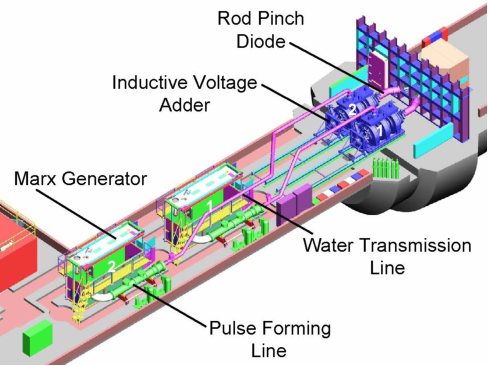
\includegraphics[width=0.75\linewidth]{cygnus_pulse_side.pdf}
\captionof{figure}{Cygnus Pulse Power Machine}
\end{center}

The Cygnus pulse power machine and imaging system is a large scale sub-critical
experiment diagnostic jointly owned and operated by Los Alamos National Labs,
Sandia National Labs, and National Securities Technologies.  An extensive data
record of thermoluminescent dosimeter (TLD) readings has been kept as a 
performance diagnostic since 2009.  From the reported dose measurements, an estimate of the radiation dose
at one meter (DAOM) from the imaged package is extrapolated based on a model of
inverse square radiation decay. 
%\end{multicols}

%------------------------------------------------

%\begin{multicols}{2}
%The data present certain challenges that make a rigorous statistical analysis
%somewhat non-standard due to the presence of significant measurement error and
%non-identical measurement replication.  
We investigate a model of non-identical measurements for estimating the mean and variation in
the DOAM of multiple radiation sources.  Our model also includes variation due to measurement error. 
%Sed fringilla tempus hendrerit. Vestibulum ante ipsum primis in faucibus orci
%luctus et ultrices posuere cubilia Curae; Etiam ut elit sit amet metus lobortis
%consequat sit amet in libero. Lorem ipsum dolor sit amet, consectetur
%adipiscing elit. Phasellus vel sem magna. Nunc at convallis urna. isus ante.
%Pellentesque condimentum dui. Etiam sagittis purus non tellus tempor volutpat.
%Donec et dui non massa tristique adipiscing. Quisque vestibulum eros eu.

\begin{center}
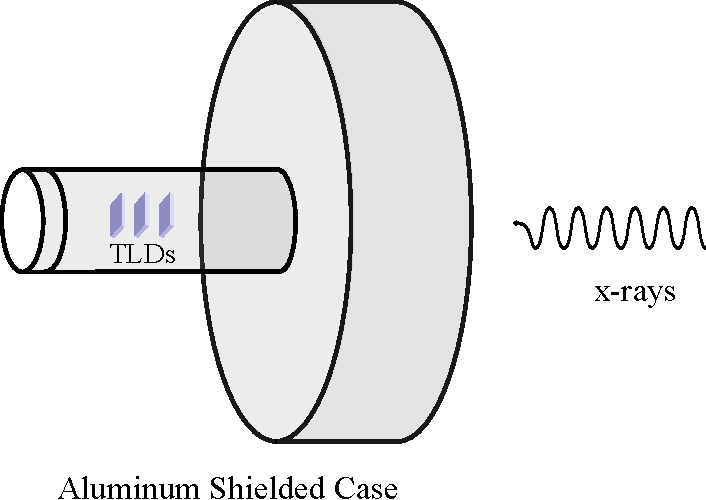
\includegraphics[width=0.75\linewidth]{tld_holder.pdf}
\captionof{figure}{TLD Measurement Device}
\end{center}

\end{multicols}
}

%----------------------------------------------------------------------------------------
%	Model
%----------------------------------------------------------------------------------------

\headerbox{Data}{name=data,column=2,row=0,bottomaligned=introduction}{

The TLD chips are stacked facing the radiation source so that the absorbed
ionizing radiation is attenuated by consecutive chips.  That is, chips stacked
behind other chips absorb less radiation and under-report dose.

\begin{center}
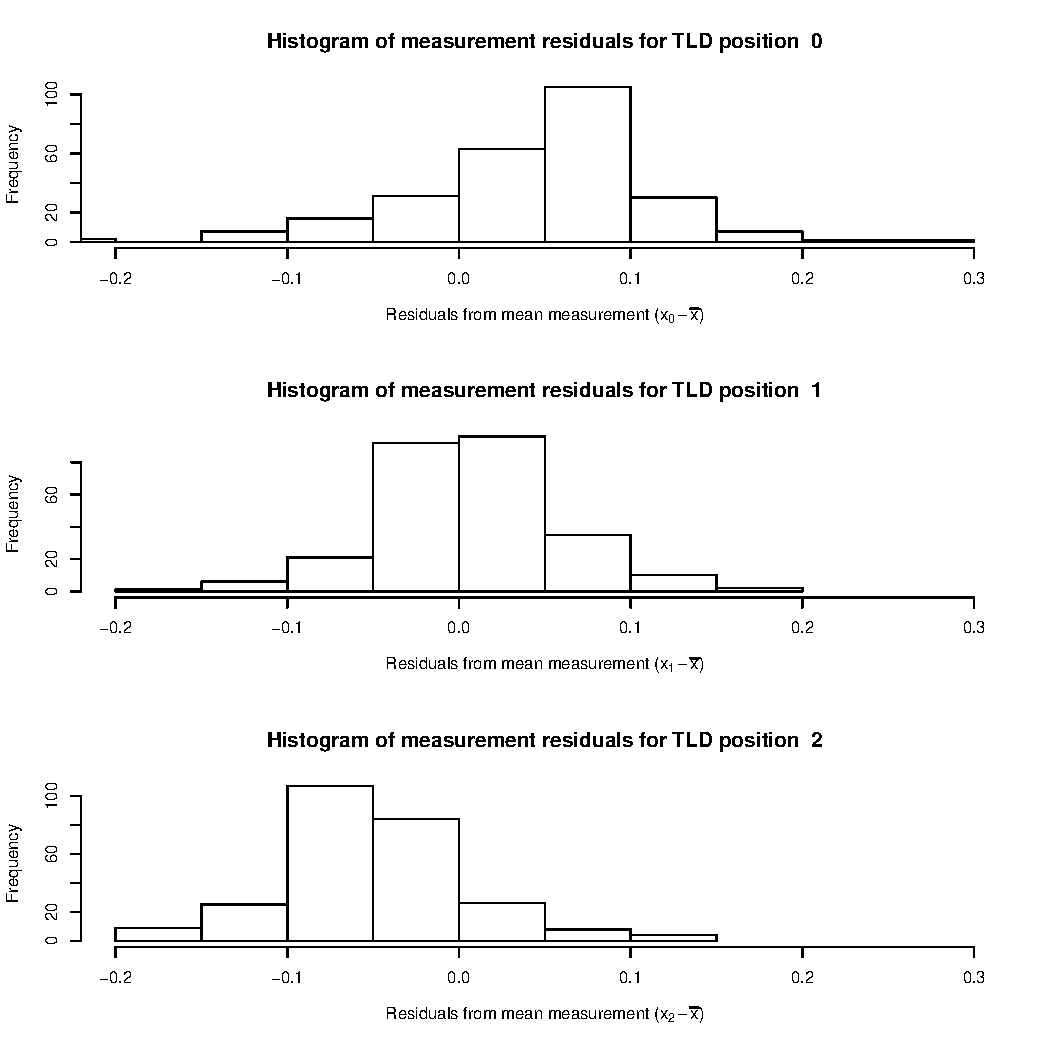
\includegraphics[width=0.65\linewidth]{attenuation.pdf}
\captionof{figure}{Evidence of Attenuation}
\end{center}


%\begin{enumerate}\compresslist
%\item Feugiat vitae elit
%\item bibendum ante sed lacinia eros in
%\item Curabitur scelerisque arcu consequat varius
%\item Dapibus nulla id purus consectetur
%\item Fringilla integer 
%\end{enumerate}
%
%\vspace{0.3em} % When there are two boxes, some whitespace may need to be added if the one on the right has more content
}

%----------------------------------------------------------------------------------------
%	Statistical Model
%----------------------------------------------------------------------------------------

\headerbox{Model}{name=model,column=3,row=0,bottomaligned=data}{
We model the TLD measurements as
proportional to the integrated energy intensity of the x-rays absorbed by the
TLD with exponential attenuation through the chips. 
\begin{equation}
  \widetilde y_{ijk} = \exp\left( \beta_{0k} + \beta_1 x_{i1} + \beta_2 x_{i2} + \eta_{ik} + \epsilon_{ijk} \right). \label{exp_model}
\end{equation}$\epsilon_{ijk}\stackrel{iid}{\sim} N(0,\sigma_\epsilon^2)$ is the random error due to TLD measurement; and $\eta_{ik} \sim N(0,\sigma_{\eta k}^2)$ is the random variation in each machine source.

A log transformation of \eqref{exp_model} results in a linear model
in the parameters with two random components. The matrix-vector form is
\begin{equation}
\vect y = \vect{X \beta} + \vect{P \eta} + \vect \epsilon, \label{matmodel}
\end{equation}
where $\vect P$ is a $6n \times 2n$ block matrix with $3\times 1$ blocks of ones along the diagonal.

}

%----------------------------------------------------------------------------------------
%	REFERENCES
%----------------------------------------------------------------------------------------

\headerbox{References}{name=references,column=0,above=bottom}{

\renewcommand{\section}[2]{\vskip 0.05em} % Get rid of the default "References" section title
\nocite{*} % Insert publications even if they are not cited in the poster
\footnotesize{ % Reduce the font size in this block
\bibliographystyle{unsrt}
\bibliography{sample} % Use sample.bib as the bibliography file
}}

%----------------------------------------------------------------------------------------
%	FUTURE RESEARCH
%----------------------------------------------------------------------------------------

\headerbox{Future Research}{name=futureresearch,column=1,span=2,aligned=references,above=bottom}{ % This block is as tall as the references block

\begin{multicols}{2}
Standard errors for the estimates on the real data still need to be estimated to obtain confidence intervals for each estimate.  These can be obtained through bootstrapping will address questions about whether the parameters actually differ from one source to the other.  More questions like these can be explored through the random effects veiwpoint.

%Maecenas viverra ligula a risus blandit vel tincidunt est adipiscing. Suspendisse mollis iaculis sem, in \emph{imperdiet} orci porta vitae. Quisque id dui sed ante sollicitudin sagittis.
\end{multicols}
}

%----------------------------------------------------------------------------------------
%	CONTACT INFORMATION
%----------------------------------------------------------------------------------------

\headerbox{Contact Information}{name=contact,column=3,aligned=references,above=bottom}{ % This block is as tall as the references block

\begin{description}\compresslist
\item[Web] www.math.umt.edu/joyce
\item[Email] kevin1.joyce@umontana.edu
%\item[Phone] +1 (000) 111 1111
\end{description}
}

%----------------------------------------------------------------------------------------
%	Results   
%----------------------------------------------------------------------------------------

\headerbox{Simulation Results}{name=results,column=2,span=2,row=0,below=data,above=references}{

\begin{multicols}{3}
\begin{center}
%{\bf Simulation Coefficients }

{\small
\renewcommand{\arraystretch}{1.2}
\begin{tabular}{|l|l|l|}
\hline
\multicolumn{3}{|c|}{TLD measurements}\\
\hline
    Variation           & $\sigma_\epsilon^2$ & 1.00e-06 \\ \hline
    Attenuation 1 & $\beta_1$           & --0.002    \\ \hline
    Attenuation 2 & $\beta_2$           & --0.004    \\ \hline
\end{tabular}

\renewcommand{\arraystretch}{1.2}
\begin{tabular}{|l|l|l|}
\hline
\multicolumn{3}{|c|}{TLD measurements}\\
\hline
    Est. Variation     & $\widehat{\sigma_\epsilon}^2$ & 6.73e-07  \\ \hline
    Est. Atten. 1 & $\widehat{\beta_1}$           &--1.98e-03 \\ \hline
    Est. Atten. 2 & $\widehat{\beta_2}$           &--3.90e-03 \\ \hline
\end{tabular}

\begin{tabular}{|l|l|l|}
\hline
\multicolumn{3}{|c|}{TLD measurements}\\
\hline
    Est. Variation     & $\widehat{\sigma_\epsilon}^2$ & 1.01e-06  \\ \hline
    Est. Atten. 1 & $\widehat{\beta_1}$           &--1.98e-03 \\ \hline
    Est. Atten. 2 & $\widehat{\beta_2}$           &--3.90e-03 \\ \hline
\end{tabular}
}

\end{center}
\end{multicols}

\begin{multicols}{3}
\begin{center}
{\small 
\renewcommand{\arraystretch}{1.2}
\begin{tabular}{|l|l|l|}
\hline
\multicolumn{3}{|c|}{Cygnus - 1 DAOM}\\
    \hline
    Mean DOAM       & $\vect{\beta_{01}}$  &1.39     \\\hline
    Variation       & $\sigma_{\eta\,1}^2$ &4.00e-04 \\\hline
\end{tabular}

\vspace{1em}
\begin{tabular}{|l|l|l|}
\hline
\multicolumn{3}{|c|}{Cygnus - 2 DAOM}\\
    \hline
    Mean DOAM & $\vect{\beta_{01}}$  &1.10     \\\hline
    Variation       & $\sigma_{\eta\,1}^2$ &0.0016   \\\hline
\end{tabular}
\captionof{table}{Simulation Coefficients.}
}

\phantom0
{\small
\renewcommand{\arraystretch}{1.2}
\begin{tabular}{|l|l|l|}
\hline
\multicolumn{3}{|c|}{Cygnus - 1 DAOM}\\
    \hline
   Est. Mean & $\vect{\widehat\beta_{01}}$   & 1.38\\\hline
    Variation       & $\widehat{\sigma}_{\eta,1}^2$ & 4.42e-04\\\hline
\end{tabular}

\vspace{1em}
\begin{tabular}{|l|l|l|}
\hline
\multicolumn{3}{|c|}{Cygnus - 2 DAOM}\\
    \hline
   Est. Mean & $\vect{\widehat\beta_{02}}$   & 1.10     \\\hline
    Variation       & $\widehat{\sigma}_{\eta,1}^2$ & 1.91e-3  \\\hline
\end{tabular}
\captionof{table}{Method 1 estimates.}
}
%{\bf Method 2 }

\phantom0
{\small
\renewcommand{\arraystretch}{1.2}
\begin{tabular}{|l|l|l|}
\hline
\multicolumn{3}{|c|}{Cygnus - 1 DAOM}\\
    \hline
   Est. Mean & $\vect{\widehat\beta_{01}}$   &1.40 \\\hline
    Variation       & $\widehat{\sigma}_{\eta,1}^2$ &4.40e-04 \\\hline
\end{tabular}

\vspace{1em}
\begin{tabular}{|l|l|l|}
\hline
\multicolumn{3}{|c|}{Cygnus - 2 DAOM}\\
    \hline
   Est. Mean & $\vect{\widehat\beta_{02}}$   &1.10 \\\hline
    Variation       & $\widehat{\sigma}_{\eta,1}^2$ & 1.90e-03    \\\hline
\end{tabular}
\captionof{table}{Method 2 estimates.}
}
\end{center}
\end{multicols}
}

%----------------------------------------------------------------------------------------
%	Results 1
%----------------------------------------------------------------------------------------

\headerbox{Estimation Method 1}{name=method1,column=0,below=introduction,bottomaligned=results}{ % This block's bottom aligns with the bottom of the results block

If we consider both random pieces as one random vector $\vect \xi = \vect
\epsilon + \vect P\vect \eta$, then we view the model as
\begin{equation}
  \vect y = \vect{X\beta} + \vect \xi, \label{matmodel2}
\end{equation}
where $\vect \xi \sim \NN(\vect 0,\vect \Sigma)$ with $\vect\Sigma$ a with a specific block matrix structure.
%$$
%\vect \Sigma = \begin{bmatrix}
%    \vect{B_1}  &             &             &  \\
%                & \ddots      &             &  \\
%                &             & \vect{B_2}  &  \\
%                &             &             & \ddots \\
%\end{bmatrix},\quad
%  \vect B_k = 
%  \renewcommand{\arraystretch}{1.2}
%  \begin{bmatrix}
%    \sigma_{\eta k}^2 + \sigma_\epsilon^2 & \sigma_{\eta k}^2 & \sigma_{\eta k}^2 \\
%    \sigma_{\eta k}^2 & \sigma_{\eta k}^2 + \sigma_\epsilon^2 & \sigma_{\eta k}^2 \\
%    \sigma_{\eta k}^2 & \sigma_{\eta k}^2 & \sigma_{\eta k}^2 + \sigma_\epsilon^2 \\
%  \end{bmatrix}.
%$$
We use an iterative generalized least squares (GLS) to estimate each of the parameters.
\begin{enumerate}
  \compresslist
  \item Initially estimate $\vect{\widehat\beta_0}$ and $\vect{\widehat \Sigma_0}$ with standard least squares.
  \item Estimate $\vect {\widehat \Sigma_k}$.  
  \item Estimate $\vect {\widehat \beta_k}$.
  \item If convergence in $\vect{\widehat \xi}_k^T \vect{\widehat \xi}_k$ is reached, stop, else set $k= k+1$ and continue from step 2.
\end{enumerate}
\hrule
\vspace{1em}
}

%----------------------------------------------------------------------------------------
%	RESULTS 2
%----------------------------------------------------------------------------------------

\headerbox{Estimation Method 2}{name=method2,column=1,below=introduction,bottomaligned=results}{ % This block's bottom aligns with the bottom of the results block
We can view \eqref{matmodel} as a mixed effects model and estimate each of the
parameters of interest using restricted maximum likelihood (REML) techniques
\cite{faraway}.  That is, we view the variation shot to shot as a random effect.

This method was implemented from codes from the \texttt{R} library
\texttt{lme4}, and the results from it are very recent.  Hence, the details of
the implementation are not known well by us, but seem to produce a less
biased estimate for the measurement variation. }

%----------------------------------------------------------------------------------------

\end{poster}

\end{document}
